% ------------------------------------------------------------------------------
% TYPO3 Version 10.1 - What's New (French Version)
%
% @license	Creative Commons BY-NC-SA 3.0
% @link		https://typo3.org/help/documentation/whats-new/
% @language	French
% ------------------------------------------------------------------------------

\section{Introduction}
\begin{frame}[fragile]
	\frametitle{Introduction}

	\begin{center}\huge{Introduction}\end{center}
	\begin{center}\huge{\color{typo3darkgrey}\textbf{Les faits}}\end{center}

\end{frame}

% ------------------------------------------------------------------------------
% TYPO3 Version 10.1 - The Facts

\begin{frame}[fragile]
	\frametitle{Introduction}
	\framesubtitle{TYPO3 Version 10.1 - Les faits}

	\begin{itemize}
		\item Date de sortie~: 01 octobre 2019
		\item Type de sortie~: Sprint Release
	\end{itemize}

	\begin{figure}
		
\includegraphics[width=0.95\linewidth]{Introduction/typo3-v10-1-banner.png}
	\end{figure}

\end{frame}

% ------------------------------------------------------------------------------
% TYPO3 Version 10.1 - Executive Summary

\begin{frame}[fragile]
	\frametitle{Introduction}
	\framesubtitle{En Résumé}

	\small
		La version 10.1 de TYPO3 est la deuxième itération sur la route de
		la version LTS (support long-terme) prévue en 2020.

		\vspace{0.2cm}

		Cette nouvelle itération comporte plus de 240 commits (changements
		de code revus, testés et approuvés) depuis la publication de la
		version précédente il y a 10 semaines.

		\vspace{0.2cm}

		Même si les utilisateurs backend ne verrons pas de changements évidents ou de
		nouvelles fonctions majeurs en l'état, le version 10.1 de TYPO3 a reçu de
		nombreuses améliorations sous le capot.

	\normalsize

\end{frame}

% ------------------------------------------------------------------------------
% System Requirements

\begin{frame}[fragile]
	\frametitle{Introduction}
	\framesubtitle{Configuration requise}

	\begin{itemize}
		\item Version de PHP~: 7.2 ou 7.3
		\item Configuration PHP~:

			\begin{itemize}
				\item \texttt{memory\_limit} >= 256M
				\item \texttt{max\_execution\_time} >= 240s
				\item \texttt{max\_input\_vars} >= 1500
				\item L'option de compilation \texttt{-}\texttt{-disable-ipv6}
					\underline(NE) doit \underline{PAS} être utilisée
			\end{itemize}

		\item La majorité des serveurs de base de données supportés par \textbf{Doctrine DBAL}
			fonctionnent avec TYPO3. Les moteurs testés sont par exemple~:
	\end{itemize}

	\begin{figure}
		
\includegraphics[width=0.80\linewidth]{Introduction/logo-databases.png}
	\end{figure}

\end{frame}

% ------------------------------------------------------------------------------
% Development, Release and Maintenance Timeline

\begin{frame}[fragile]
	\frametitle{Introduction}
	\framesubtitle{Chronologie des développements, sorties et maintenances}

	\textbf{TYPO3 v10}

	\begin{figure}
		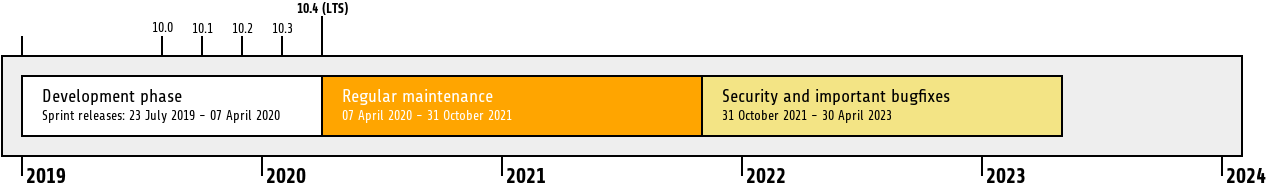
\includegraphics[width=1\linewidth]{Introduction/typo3-v10-lifecycle.png}
	\end{figure}

	\textbf{Support étendu}\newline
	\smaller
		\href{https://typo3.com}{TYPO3 GmbH} propose des options de support pour TYPO3
		v10 LTS même après de 30 Avril 2023, pour 2 ans supplémentaires maximum.
	\normalsize

\end{frame}

% ------------------------------------------------------------------------------
% TYPO3 v10 Roadmap

\begin{frame}[fragile]
	\frametitle{Introduction}
	\framesubtitle{Feuille de route TYPO3 v10}

	Dates de sortie et objectifs principaux~:

	\begin{itemize}

		\item v10.0 \tabto{1.1cm}23/Jui./2019\tabto{3.4cm}Ouvre la voie à de nouveaux concepts et APis
		\item
			\begingroup
				\color{typo3orange}
				v10.1 \tabto{1.1cm}01/Oct./2019\tabto{3.4cm}Améliorations routage et gestion des sites V2
			\endgroup
		\item v10.2 \tabto{1.1cm}03/Déc./2019\tabto{3.4cm}Améliorations du moteur de rendu Fluid
		\item v10.3 \tabto{1.1cm}04/Fév./2020\tabto{3.4cm}Gèle des fonctionnalités
		\item v10.4 \tabto{1.1cm}07/Avr./2020\tabto{3.4cm}Version LTS (Long-term Support)

	\end{itemize}

	\smaller
		\url{https://typo3.org/article/typo3-v10-roadmap/}\newline
		\url{https://typo3.org/article/typo3-v10-safe-and-sound/}
	\normalsize

\end{frame}

% ------------------------------------------------------------------------------
% Installation

\begin{frame}[fragile]
	\frametitle{Introduction}
	\framesubtitle{Installation}

	\begin{itemize}
		\item Procédure officielle \textit{classique} d'installation sous Linux/Mac OS X\newline
			(DocumentRoot considéré \texttt{/var/www/site/htdocs})~:
		\begin{lstlisting}
$ cd /var/www/site
$ wget --content-disposition get.typo3.org/10.1
$ tar xzf typo3_src-10.1.0.tar.gz
$ cd htdocs
$ ln -s ../typo3_src-10.1.0 typo3_src
$ ln -s typo3_src/index.php
$ ln -s typo3_src/typo3
$ touch FIRST_INSTALL
		\end{lstlisting}

		\item Liens symboliques sous Microsoft Windows~:

			\begin{itemize}
				\item Utiliser \texttt{junction} sous Windows XP/2000
				\item Utiliser \texttt{mklink} sous Windows Vista et Windows 7 ou supérieur
			\end{itemize}

	\end{itemize}
\end{frame}

% ------------------------------------------------------------------------------
% Installation using composer

\begin{frame}[fragile]
	\frametitle{Installation and Upgrade}
	\framesubtitle{Installation avec \texttt{composer}}

	\begin{itemize}
		\item Installation avec \textit{composer} sous Linux, Mac OS X et Windows 10~:

			\begin{lstlisting}
$ cd /var/www/site/
$ composer create-project typo3/cms-base-distribution typo3v10 ^10.1
			\end{lstlisting}

		\item Vous pouvez aussi créer votre ficher \texttt{composer.json} sur mesure
			et exécuter~:

			\begin{lstlisting}
$ composer install
			\end{lstlisting}

			Plus de détails et exemples de fichiers \texttt{composer.json} disponibles à~:\newline
			\smaller
				\href{https://composer.typo3.org}{https://composer.typo3.org}
			\normalsize

	\end{itemize}
\end{frame}

% ------------------------------------------------------------------------------
